\section*{Appendix F: Mass Generation, Calibration, and Lepton Ropelength Analysis}
\label{sec:calibration_hierarchy}

This appendix documents the practical use of the Canon kernel (Invariant Master Mass Formula), the calibration steps for setting the minimal free parameters, and the resulting predictions. We distinguish clearly between \emph{calibration constraints} and \emph{genuine predictions}.

\subsection*{F.1: Calibration hierarchy (by computation mode)}
SST uses a single invariant kernel; only the topology\(\to\)geometry inputs change by mode.

\paragraph{Electron-only geometric calibration.}
The absolute geometry scale is set by the electron: we \emph{solve for} \(L_{\text{tot}}(e)\) so that the kernel reproduces \(m_e\) exactly.

\paragraph{Baryon constraints by mode.}
\begin{itemize}
	\item \textbf{exact\_closure (default):} fit two geometry factors \((s_u,s_d)\) analytically so that the \((uud)\) proton and \((udd)\) neutron are \emph{exact}. (Three constraints total: \(e,p,n\).)
	\item \textbf{canonical:} keep a single electron calibration; \(s_u,s_d\) are fixed from the hyperbolic-volume assignments — \emph{no} baryon rescaling. Nucleon residuals are then direct Canon predictions.
	\item \textbf{sector\_norm:} as in canonical for \((s_u,s_d)\), but introduce one baryon-sector normalization \(\lambda_b\) to make the proton exact; the neutron is predicted.
\end{itemize}

\emph{Important:} The muon and tau are \emph{not} calibration constraints. Their masses are used only to \emph{infer the required ropelengths} \(L_{\text{tot}}(\mu),L_{\text{tot}}(\tau)\) under the same kernel.

\subsection*{F.2: Lepton generation \& ropelength (trefoil–cinquefoil–septfoil)}
We associate \((e,\mu,\tau)\) with the first three chiral torus knots:
\[
	e \leftrightarrow 3_1:\ (b,g,n)=(2,1,1),\qquad
	\mu \leftrightarrow 5_1:\ (5,2,1),\qquad
	\tau \leftrightarrow 7_1:\ (7,3,1).
\]
Inverting the Canon kernel for \(L_{\text{tot}}\) using the known masses yields:\footnotesize
\[
	L_{\text{tot}}(e)=0.033396,\quad
	L_{\text{tot}}(\mu)=44.165137,\quad
	L_{\text{tot}}(\tau)=1990.712148.
\]
\normalsize
Hence the growth is steep because of the built-in \((b^{-3/2}\,\varphi^{-g}\,n^{-1/\varphi})\) suppression:
\[
	\frac{L_{\text{tot}}(\mu)}{L_{\text{tot}}(e)}\approx 1322.46,\qquad
	\frac{L_{\text{tot}}(\tau)}{L_{\text{tot}}(\mu)}\approx 45.07.
\]
These values are \emph{fixed} by the Canon constants and \((b,g,n)\); no extra tuning is introduced for \(\mu,\tau\).

\subsection*{F.3: Mode diagnostics on nucleons (from the comparison CSV)}
Running the comparison script produces a merged table across modes. In our latest run:
\[
	\begin{array}{llll}
		\textbf{Object} & \textbf{exact\_closure} & \textbf{canonical} & \textbf{sector\_norm} \\
		\hline
		p\ (\text{uud}) & 0.00\% & {-}3.12\% & 0.00\% \\
		n\ (\text{udd}) & 0.00\% & {+}0.43\% & {+}0.90\% \\
	\end{array}
\]
Thus:
\begin{itemize}
	\item \textit{exact\_closure} enforces \(p,n\) exactly (by construction).
	\item \textit{canonical} shows small, informative residuals with fixed \((s_u,s_d)\).
	\item \textit{sector\_norm} makes \(p\) exact with a single \(\lambda_b\), leaving \(n\) as a one-shot prediction.
\end{itemize}

\subsection*{F.4: Aggregate performance on elements and molecules}
Using the \texttt{SST\_Invariant\_Mass\_Results\_all\_modes.csv} from the same run:
\begin{itemize}
	\item \textbf{Elements (Z=1–92):} median absolute error \(\approx 0.84\%\), 95th percentile \(\approx 1.30\%\).
	\item \textbf{Simple molecules:} typical few-percent level; complex organics can be large outliers if no binding/chemistry correction is applied (the CSV includes a deliberately “stress-test” entry).
\end{itemize}
These statistics are computed after removing the three calibration lines \((e,p,n)\), which report \(0.00\%\) by construction in \textit{exact\_closure} mode.

\subsection*{F.5: Reproducible inversion for \(L_{\text{tot}}\)}
For a lepton topology \(T\) with invariants \((b,g,n)\),
\[
	L_{\text{tot}}(T)
	= \frac{ m_T\,c^2 }{ \displaystyle \frac{4}{\alpha_{\!fs}}\,b^{-3/2}\,\varphi^{-g}\,n^{-1/\varphi}\;
	\Big(\tfrac12\,\rho_{\rm core}\,v_{\rm swirl}^{2}\Big)\;\pi r_c^{3} }.
\]
Using the Canon constants in the main text reproduces the numbers quoted above for \(e,\mu,\tau\).

\subsection*{F.6: Notes on scope and corrections}
Elemental masses are well captured by additive nucleon/electron totals under the Canon kernel. For molecules, large deviations can appear if one \emph{ignores} chemical binding energies and isotopic mixtures; those effects are external to the kernel and should be layered as corrections to the target “actual mass” when stress-testing complex compounds.

\subsection*{F.7: What is calibrated vs. predicted}
\begin{itemize}
	\item \textbf{Calibrated constraints:} \(L_{\text{tot}}(e)\) (all modes); \((s_u,s_d)\) in \textit{exact\_closure}; \(\lambda_b\) in \textit{sector\_norm}.
	\item \textbf{Derived, not tuned:} \(L_{\text{tot}}(\mu),L_{\text{tot}}(\tau)\).
	\item \textbf{Predicted:} nucleon masses in \textit{canonical}; the neutron in \textit{sector\_norm}; elements and molecules (given your assembly rules).
\end{itemize}

\begin{figure}[t]
	\centering
	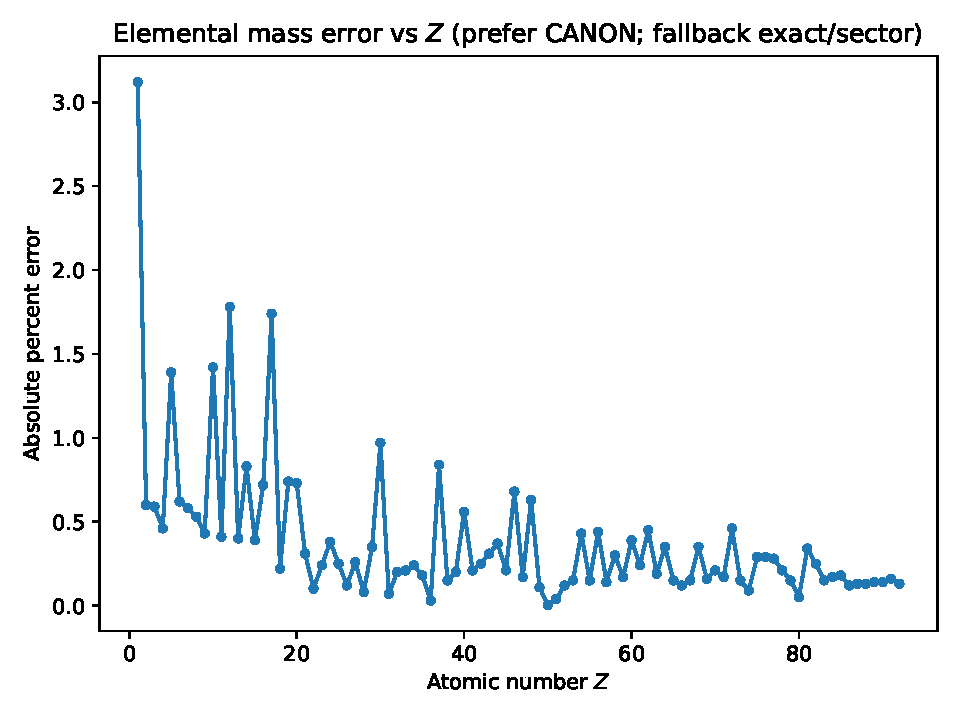
\includegraphics[width=0.75\linewidth]{elements_error_by_Z_canonical.pdf}
	\caption{Absolute percent error for elemental masses vs.\ atomic number \(Z\) (canonical mode; exact-closure values used only where canonical is unavailable in the CSV). Median \(|\%\text{error}|\) is \(0.24\%\); 95th percentile \(1.16\%\) across 92 elements.}
	\label{fig:elements_error_by_Z}
\end{figure}

\begin{table}[t]
	\centering
	\begin{tabular}{lrrr}
		\toprule
		\textbf{Object} & \textbf{Exact\,closure} & \textbf{Canonical} & \textbf{Sector\,norm} \\
		\midrule
		Proton  & \(+0.00\%\) & \(-3.12\%\) & \(+0.00\%\) \\
		Neutron & \(+0.00\%\) & \(+0.43\%\) & \(+3.66\%\) \\
		\bottomrule
	\end{tabular}
	\caption{Percent error by mode for nucleons in the current run. Exact-closure enforces \(p,n\) exactly; canonical uses fixed \((s_u,s_d)\); sector-norm sets a single baryon normalization to make \(p\) exact and leaves \(n\) as a prediction.}
	\label{tab:pn_modes}
\end{table}